 \chapter{Methods}
 \section{Overview and Terminology}
In order to initialize PC2L for a project, one must use the singleton \texttt{System} class, which contains system-wide settings, information, and shared objects. Settings on this class will determine the number of nodes that should be used in a run of PC2L. After this class is successfully obtained, the user can start PC2L, use data structures and algorithms, and then close PC2L when its features are no longer necessary, terminating all distributed processes. In this way, PC2L can be easily integrated into any portion of an existing application, allowing users to trivially transition from serial execution on one machine to distributed computing, then back to serial computing again if necessary. In any given instance of PC2L, there can be an arbitrary number of distributed \texttt{Worker} objects which handle the message passing work that would typically be done by users in a traditional distributed computing workflow. PC2L also includes a mode in which only one node in a cluster can write data, while the rest of the nodes are used as a distributed cache. This mode of operation allows for maximal utilization of cluster-wide memory and eliminates the potential for write-collisions, making it useful for applications in which a large in-memory data structure is constructed then queried many times. 

\subsection{Message Passing}
The main goal of this thesis is to deliver a portable library for parallel/distributed computing that is optimized for working with data intensive applications. In order to achieve this, we need some form of communication across nodes in a supercomputing cluster and/or processes on a local machine. Instead of reinventing the wheel by developing our own message passing protocol, we will stick with the industry standard Message Passing Interface (MPI) \cite{mpi}. MPI was standardized by 60 people from 40 top computing organizations across the United States including researchers, computer manufacturers, laboratories, and major companies. Nine versions of MPI have come out since the protocol's debut in 1994, with varying degrees of acceptance and adoption from the supercomputing community, but its core functionality is used almost universally in all high performance computing projects. Despite MPI's status as the \textit{de facto} standard for message passing, other alternatives to MPI that have gained more popularity in industry. Among these are Spark \cite{spark}, Charm++ \cite{parallel_programming_w_charm}, and ARMCI \cite{ARMCI}. However, Charm++ is actually an abstraction over MPI, utilizing it is a hidden backend, ARMCI does not deliver nearly all of the same features as the MPI standard, and, as demonstrated by one recent study of a big memory application in metagenomics \cite{metagenomics}, MPI applications are typically much faster and much less memory hungry than their Spark equivalents. 

In PC2L, the main purposes for message passing will be memory synchronization among nodes and instruction delivery to distributed workers. For instance, a \texttt{pc2l::Vector} may be stored across several nodes, with distinct or overlapping sub-vectors in each node. If a program is operating on only one section of the vector corresponding to only one node, these changes can be stored in a node-level cache initially, then any caches storing the same data, along with workers operating on this data, can be informed of changes via an update message.  

\subsection{Message Class}
Instead of directly interfacing with an MPI implementation through the typical MPI directives, PC2L utilizes a \texttt{Message} class for internal consumption that abstracts most of these features away. This level of abstraction allows the underlying MPI commands to be changed without modifying the code in every single file across PC2L. Additionally, it opens the door for version of PC2L that are compatible with different versions of MPI, perhaps utilizing some more recently features in different versions. All of the MPI commands utilized in PC2L are redefined as macros within an internal MPI-helper header. 

\subsection{Workers}
Classes that inherit the \texttt{Worker} interface are used to abstract away different kinds of message passing in PC2L. At a minimum, any class that implements the \texttt{Worker} interface runs on a process with non-zerio MPI rank, sends messages to other \texttt{Worker} classes, and contains a buffer used to keep track of received messages. Workers will initially only be concerned with storing and retrieving information from a PC2L instance's distributed Cache, but different \texttt{Worker} variations will likely be added as the project progresses and different needs arise. 

\subsection{CacheWorker} 
A \texttt{CacheWorker} in PC2L is responsible for sending and receving cache-blocks to and from different processes. In order to best utilize the RAM in each separate node, each \texttt{CacheWorker} process will be run on a different compute node. When a \texttt{CacheWorker} is sent a message to store or retrieve a block of data, it will compute a composite key that combines that data structure type within which the block is stored with a unique block tag generated at run-time, allowing for $\mathcal{O}(1)$ address retrieval for members within a given distributed container. 
\subsection{CacheManager}
While there is one \texttt{CacheWorker} for every node included in a run of PC2L, there is only one \texttt{CacheManager} overall system-wide. The \texttt{CacheManager} for a given run of PC2l will run on the process with MPI rank zero, and will coordinate each \texttt{CacheWorker} across the system. Data structures in the program will communicate with the \texttt{CacheManger}, which will then schedule tasks to be performed on one of the many \texttt{CacheWorkers} using message passing.  


The library includes two data structures, \texttt{pc2l::Vector} and \texttt{pc2l::Map} which work the same way as their standard library equivalents. In order to relay information between machines on an interconnected computing cluster, MPI. A single write-back cache on the \texttt{CacheManager} node (MPI rank 0) is utilized, and memory is moved to the connected \texttt{CacheWorker} nodes as soon as the RAM space on the head node is exceeded. The code for the library is publicly available on github at \url{https://github.com/rudiejd/pc2l}, and it is intended to be used as a static shared library. Additionally, we have provided several applications which illustrate how PC2L might be used. Other than including some wind-up code which ensures that MPI is correctly initialized and terminated, data structures within the library can be used in exactly the same fashion as those in the libstdc++ STL.

\paragraph{Code sample}
This code solves the first project euler problem, which asks for the sum of all numbers below $n$ that are multiples of 3 or 5. \cite{euler_1}. Compare to the STAPL code mentioned in Chapter 2.
\scriptsize
\begin{lstlisting}[language=C++, caption=PC2L code sample for Project Euler number 1. Headers removed for brevity, captionpos=b]

using ull = unsigned long long;

int main(int argc, char *argv[]) {
    // Boilerplate code to get MPI up and running
    auto& pc2l = pc2l::System::get();
    pc2l.initialize(argc, argv);
    pc2l.start();
    ull num = strtoull(argv[1], NULL, 0);

    // initialize a vector of type unsigned long long filled with the number specified by 2nd command line argument
    // this vector uses blocks of size 8 * sizeof(ull) = 8 * 8 = 64 bytes (on most systems)
    // Note how this value can be provided by users
    pc2l::Vector<ull, 8 * sizeof(ull)> vec(num);

    // fill vector with values from 1 to n
    std::iota(vec.begin(), vec.end(), 1);

    // every number that does not have a 3 or 5 as a factor is set to 0
    std::replace_if(vec.begin(), vec.end(), [](auto i) {
        return !((i % 3) || (i % 5));
    }, 0);

    // sum all elements in the vector
    auto total = std::accumulate(vec.begin(), vec.end(), 0ULL);

    std::cout << "The total is " << total << std::endl;

    // Boilerplate to shut down MPI
    pc2l.stop();
    pc2l.finalize();
}
\end{lstlisting}
\normalsize
\section{Architecture}
\begin{figure}[h]
\centering
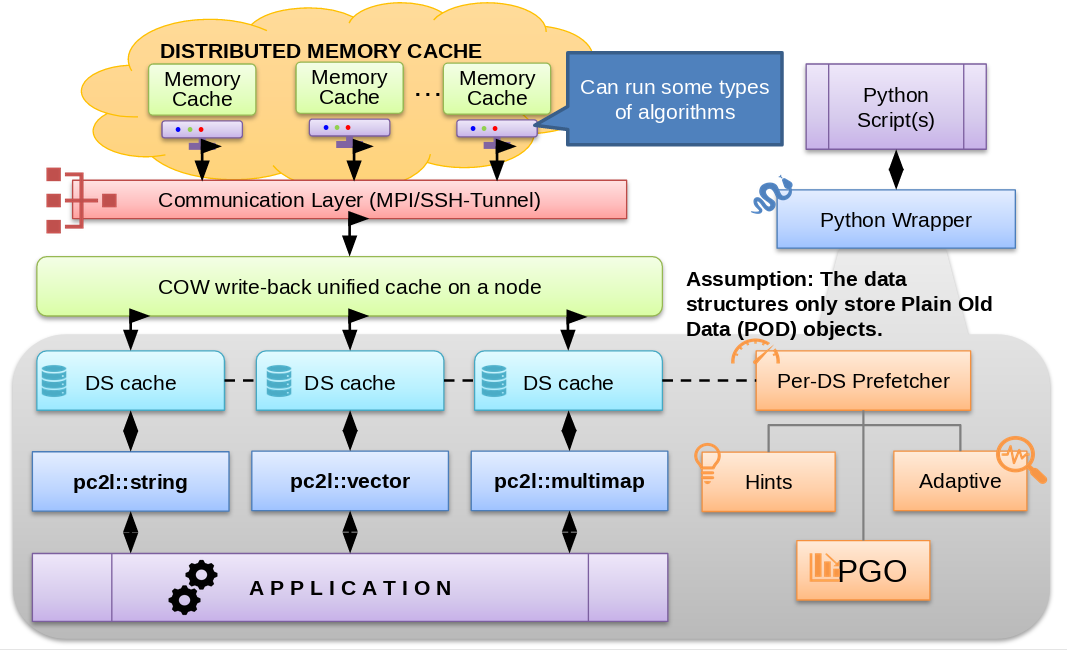
\includegraphics[width=0.65\textwidth]{Figures/pc2l_architecture.png}
\caption{Architecture of PC2L}
\label{fig:pc2l_architecture}
\end{figure}
As previously discussed, PC2L's architecture is based on a single "writer" node that serves as the cache along with networked child nodes that essentially operate in a write-back scheme. Figure \ref{fig:pc2l_architecture} displays the initial vision for how PC2L might have worked. As of the completion of this thesis,  only a COW write-back unified cache and a distributed memory cache accessed through a communication tunnel have been achieved. The data structures depicted in this initial vision have also been implemented, and some degree of rudimentary prefetching has been implemented. However, there is not currently a python wrapper for this project. Several important implementation decisions in the course of implementing this architecture include storing member data for each data structure in blocks of heterogeneous size, utilizing template metaprogramming not just for generic typing, but also to allow users to choose functionality for each data structure, custom cache eviction routines, and prefetching routines. Each one of these topics deserves more thorough exposition. 

\subsubsection{Block Division} \label{sec:block_div}
Every time an item within a PC2L data structure is retrieved or stored, there is a chance that it may need to be retrieved or sent to a remote node based on the current state of the head node. Sending individual objects would be incredibly inefficient, especially considering that a single data structure within a big memory project could potentially contain trillions of objects. As a result, the objects within a data structure are grouped into \textbf{blocks} of a user defined size. These blocks are then transferred together. For example, if a user wishes to manipulate a \texttt{pc2l::Vector} of one trillion integers ($4*10^{12}$ bytes), they might consider using blocks of size $4*10^6$ so that at least a million integers are stored in adjacent memory in one block. Performance increases from larger blocks rely on the fact that users are likely to access items in the same spatial region of a data structure, and everyapplication - even every data structure within an application - may have a different sweet spot for block size. As a result, the library allows users to set heterogeneous block sizes by changing template parameters. 
For each block within the system, a unique identifier is computed based on a combination of the data structure that generated the block and the block's relative position within said data structure. This identifier is then used within all of the caching infrastructure to uniquely identify blocks. 

\subsubsection{Cache Eviction}
Cache Eviction was another key aim of this project. Namely, providing varying cache eviction policies  which can be selected by the user to fit their application. Many cache eviction strategies were implemented by creating some sort of ordered queue (a \texttt{std::list}) which lives on the \texttt{CacheManager} node. The ordering of this queue then is defined by the selected eviction policy. For example, an LRU eviction policy would have the least recently used block at the back of the queue, with the most recently used block being placed in front of the queue. On the other hand, a time-aware LRU eviction strategy would be similar, except the queue would also have to be ordered by time to use (TTU). There are three strategies for cache eviction currently implemented in PC2L: Least Recently Used (LRU), Most Recently Used (MRU), Least Frequently Used (LFU), and Pseudo Least Recently Used (PLRU). 

\paragraph{Least Recently Used}
\begin{algorithm}
    \caption{Least Recently Used Eviction Strategy}
    \begin{algorithmic}[1]
        \State $B = \texttt{Block}$
        \State $C = \texttt{Map}$
        \State $Q = \texttt{Queue}$
        \State $n \ge 0$
        \State $m = |Q|$
        \If{$B \not \in C$} 
            \If{$\texttt{CurrentSize}(C) + \texttt{Size}(B) > n$} 
                \State $T \gets Q_m$
                \State $Q \gets Q - \{Q_m\}$\
                \State $E \gets C_T$\
                \State $M \gets M - \{C_T\}$\
                \State $\texttt{SendToRemoteCacheWorker}(E)$\
            \EndIf
        \Else
            \State $Q \gets Q - \{Q_B\}$
        \EndIf
        \State $\texttt{PushFront}(Q, B)$
    \end{algorithmic}
\end{algorithm}
The Least Recently Used eviction strategy is the default in PC2L. This implementation specifically takes a lot of influence from Johnson and Sasha's 2Q algorithm (reference here). Essentially, it aims to privilege the blocks which have appeared in the most recent calls to the cache. The main data structures of note in the algorithm illustrated above are the Queue and the cache - obviously the complexity of the algorithm is dependent on the complexity of insertion into and removal from these structures. PC2L utilizes a doubly-linked list to minimize the cost of insertion and removal from the queue. The cache is implemented using a hash-map with the unique block identifier described in \label{block_div} serving as the key, while the block servers as the value. 

\paragraph{Most Recently Used}
\begin{algorithm}
    \caption{Most Recently Used Eviction Strategy}
    \begin{algorithmic}[1]
        \State $B \gets \texttt{Block}$
        \State $C \gets \texttt{Map}$
        \State $Q \gets \texttt{Queue}$
        \State $n \ge 0$
        \State $m \gets |Q|$
        \If{$B \not \in C$} 
            \If{$\texttt{CurrentSize}(C) + \texttt{Size}(B) > n$} 
                \State $T \gets Q_1$
                \State $Q \gets Q - \{Q_1\}$\
                \State $E \gets C_T$\
                \State $M \gets M - \{C_T\}$\
                \State $\texttt{SendToRemoteCacheWorker}(E)$\
            \EndIf
        \Else
            \State $Q \gets Q - \{Q_B\}$
        \EndIf
        \State $\texttt{PushFront}(Q, B)$
    \end{algorithmic}
\end{algorithm}
In many ways, this eviction strategy is equivalent to the Least Recently Used strategy. The only key difference here is that under the Most Recently Used strategy, the blocks which have appeared in the least recent calls to the cache are privileged. This cache eviction strategy has been shown to provide significant performance increase for applications which follow looping sequential access patterns (reference here).

\paragraph{Least Frequently Used}
\begin{algorithm}
    \caption{Least Frequently Used Eviction Strategy}
    \begin{algorithmic}[1]
        \State $B \gets \texttt{Block}$
        \State $P \gets \texttt{Map}$
        \State $Q \gets \texttt{QueueOfQueues}$ 
        \State $n \ge 0$
        \State $m \gets |Q|$
        \If{$B \not \in P$} 
            \If{$\texttt{CurrentSize}(Q) + \texttt{Size}(B) > n$} 
                \State $S \gets Q_1$
                \State $m \gets |S|$
                \State $E \gets S_m$
                \State $S \gets S - \{S_m\}$
                \If{$|S| = 0$}
                    \State $Q \gets Q - \{S\}$
                \EndIf
                \State $\texttt{SendToRemoteCacheWorker}(E)$\
            \EndIf
        \Else
            \State $I \gets P_B$
            \State $IQ \gets Q_{\texttt{Frequency}(I)}$
            \State $IQ \gets IQ - \{I\}$
            \If{$|IQ| = 0$}
                \State $Q \gets Q - \{Q_{\texttt{Frequency}(I)}\}$
            \EndIf
            \State $\texttt{Frequency}(I) \gets \texttt{Frequency}(I) + 1$
            \State $Q_{\texttt{Frequency}(I)} \gets Q_{\texttt{Frequency}(I)} \cup \texttt{I}$
            \State $P_B \gets {Q_{\texttt{Frequency}(I)}}_1$
        \EndIf
        \State $\texttt{PushFront}(Q, B)$
    \end{algorithmic}
\end{algorithm}
Instead of only considering the order of calls, as with LRU variants, the Least Frequently Used strategy attempts to also privilege items which have been used many times. The algorithm described above is adapted from that which is described in (refernce to O(1) LFU algorithm). The main idea is that instead of one queue, there is now one queue for each value in the range of access frequencies for each item currently in the cache. In the event that two or more blocks are tied for the minimum frequency $m$, the LRU block in the $m$-queue will be selected. In other words, the LFU strategy falls back to LRU in the event of a tie. 


\begin{algorithm}
    \caption{Pseudo Least Recently Used}
    \begin{algorithmic}[1]
        \State $B = \texttt{Block}$
        \State $C = \texttt{Map}$
        \State $Q = \texttt{Queue}$
        \State $n \ge 0$
        \State $m = |Q|$
        \If{$B \not \in C$} 
            \If{$\texttt{CurrentSize}(C) + \texttt{Size}(B) > n$} 
                \State $T \gets Q_0$
                \State $Q \gets Q - \{Q_0\}$\
                \State $E \gets C_T$\
                \State $M \gets M - \{C_T\}$\
                \State $\texttt{SendToRemoteCacheWorker}(E)$\
            \EndIf
        \Else
            \State $Q \gets Q - \{Q_B\}$
        \EndIf
        \State $\texttt{PushFront}(Q, B)$
    \end{algorithmic}
\end{algorithm}
